
\begin{figure*}
  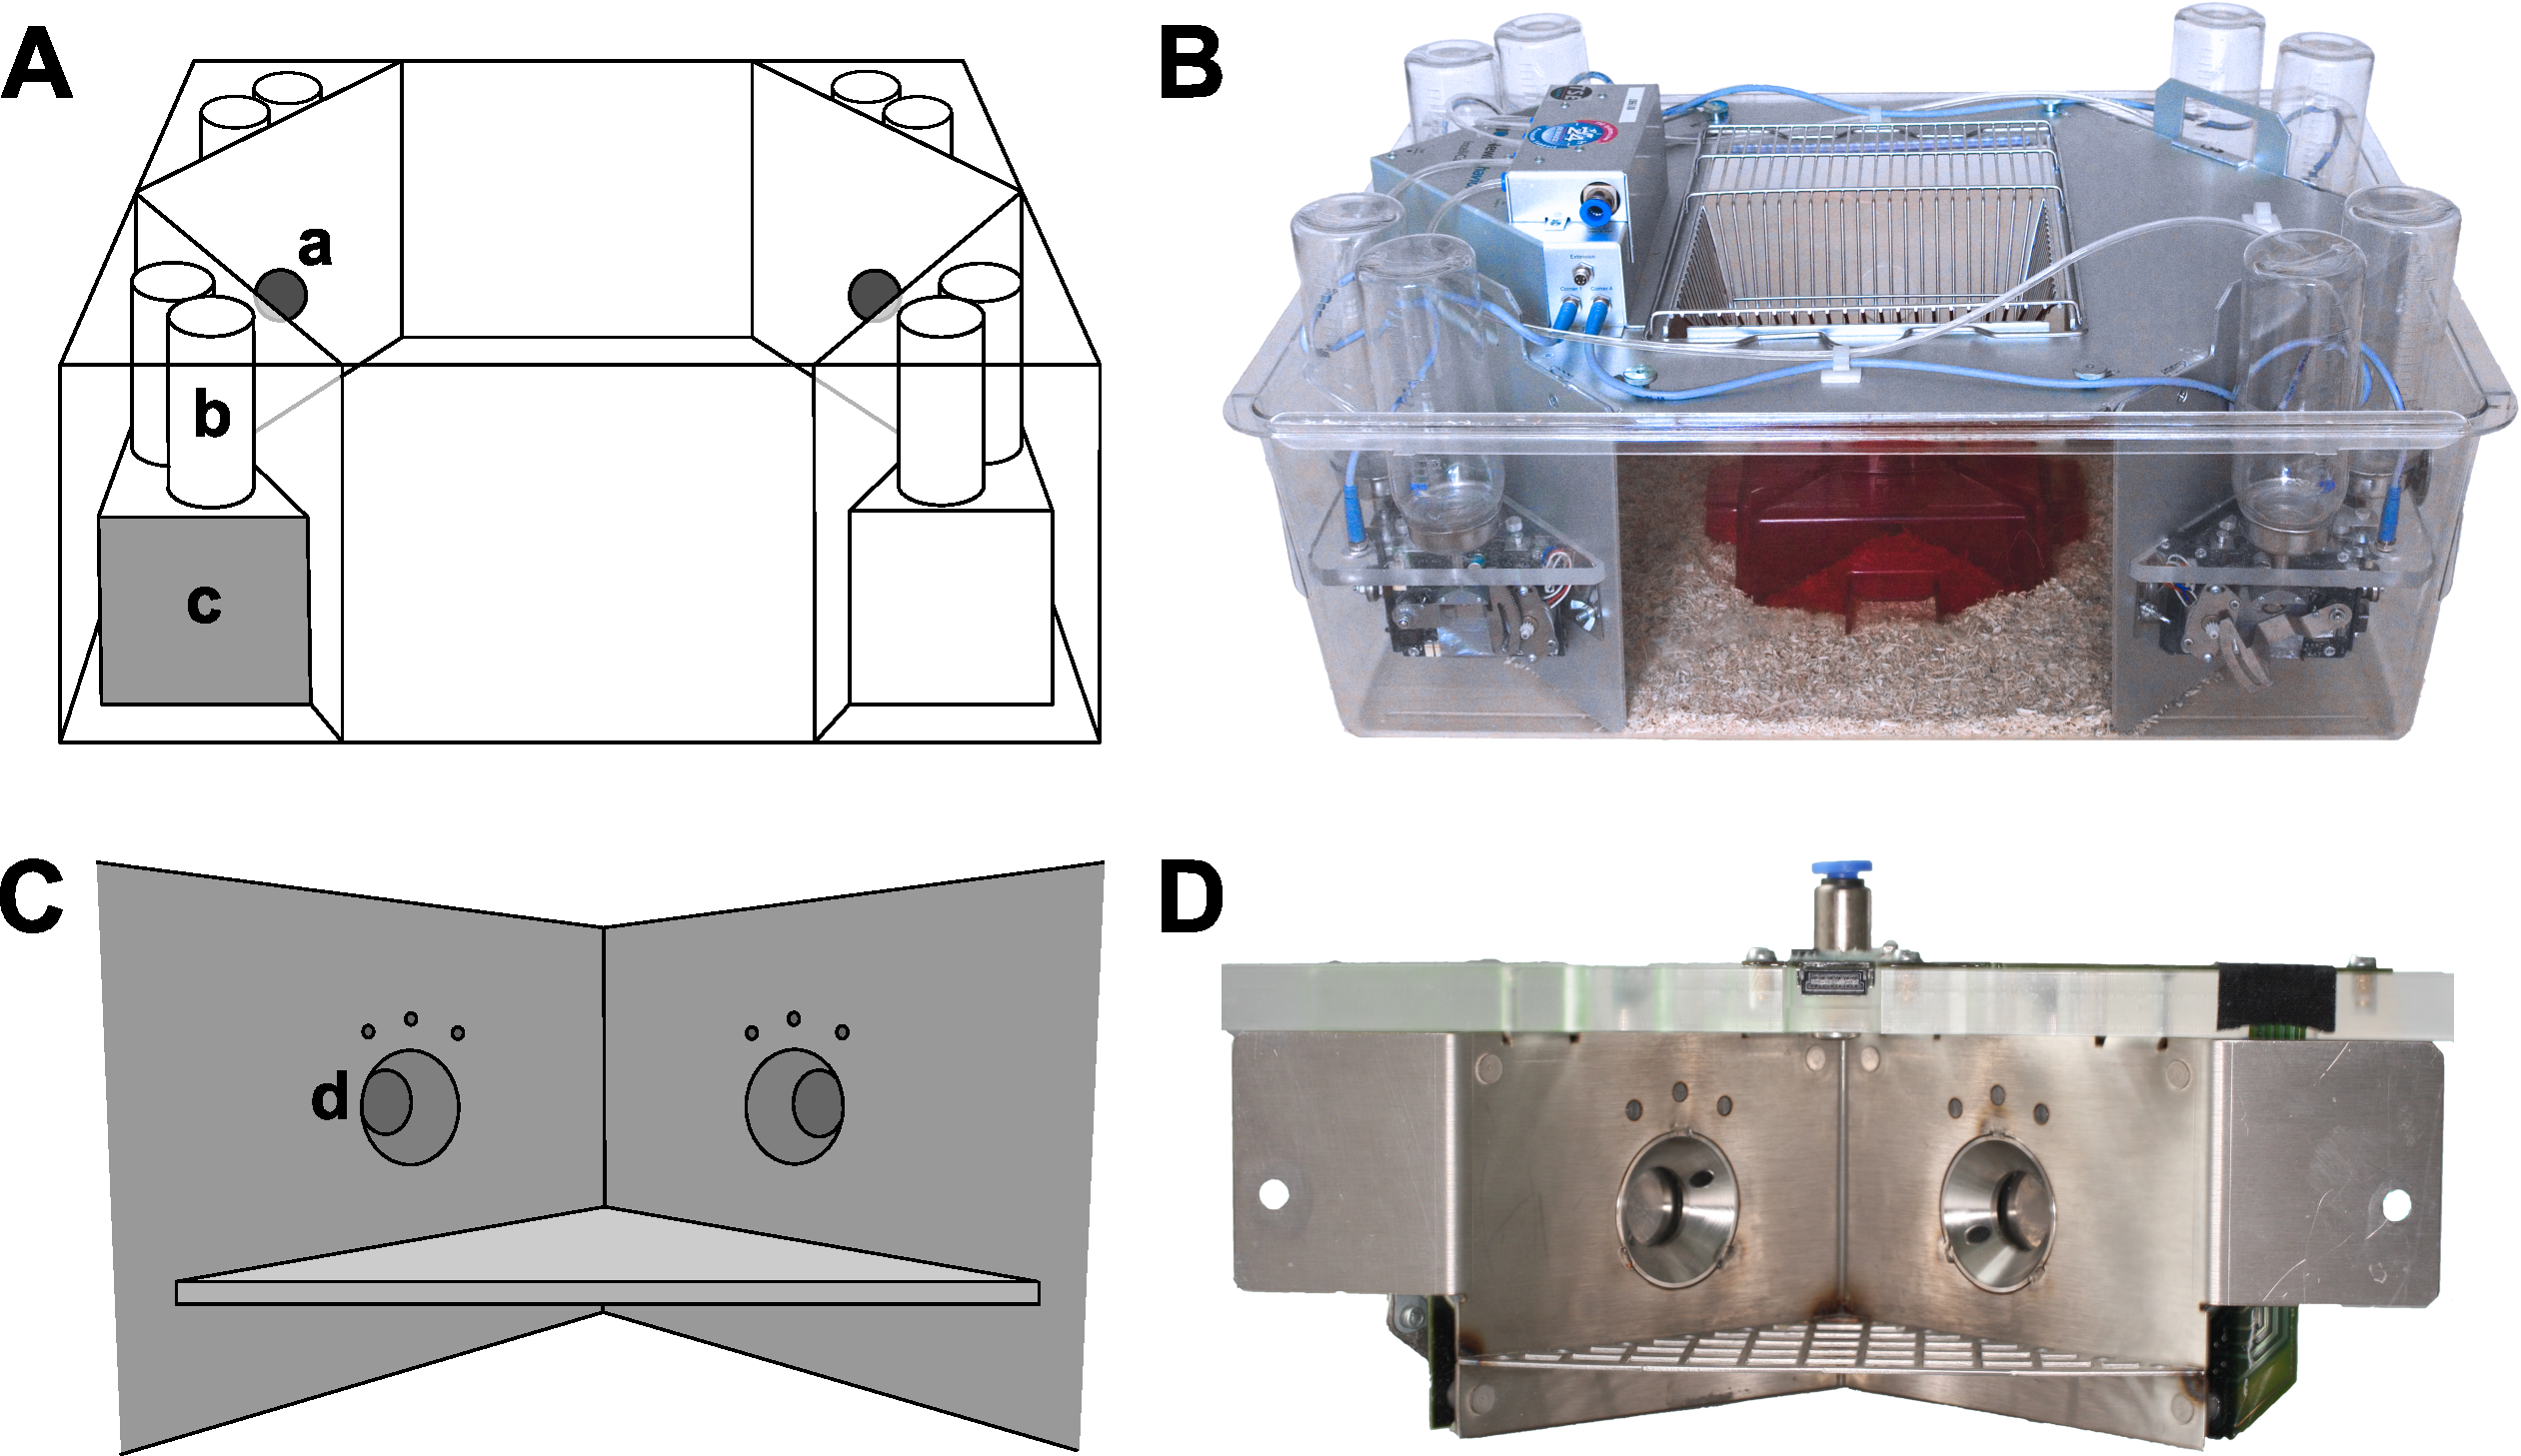
\includegraphics[width=0.75\textwidth]{figures/FigureIC.pdf}
  \caption{
    {\bf IntelliCage system.}
    The system is composed of one or more cages (A,~B).
    Through openings (a) mice can access bottles (b) in a learning chamber (c;~C,~D).
    Access to the bottles is controlled by programmable door in smaller openings in the sides
    of the chamber (d). \emph{Credits:} A, C -- Maria Nowicka, JD; B -- Anna Mirgos, D -- SŁ
  }
  \label{intellicageSystem}
\end{figure*}

IntelliCage (\fig{intellicageSystem}) is an automated, computer-controlled RFID system for
(possibly long-term) monitoring of groups of
mice~\cite{Galsworthy:2005br,Krackow:2010ck,Puscian:2014cu}. The mice are housed in
one or more polycarbonate cages (of size 55 x 37.5 x 20.5 cm;
\fig{intellicageSystem}\textbf{A},~\textbf{B}). A cage can house a group of up to
16 mice. Each mouse is tagged with an RFID transponder.

The key components of the system are learning chambers
(\fig{intellicageSystem}\textbf{c},~\textbf{C},~\textbf{D})
located in the corners of cages
(for brevity, we will refer to the chambers simply as `corners'). Each
corner can be accessed through a circular opening (30 mm in diameter; \fig{intellicageSystem}\textbf{a}),
with an embedded RFID antenna. By design, only one mouse at a time can enter
a corner. Each corner contains two smaller (13 mm in diameter; \fig{intellicageSystem}\textbf{d}) openings,
through which a mouse can access different drinking bottles (\fig{intellicageSystem}\textbf{b}). The access to the
drinking bottles is controlled using programmable doors in
the smaller openings.


A broad range of different experiment protocols can be implemented in the
IntelliCage~\cite{Knapska:2006cz,Kiryk:2011tk,Endo:2011bs,Radwanska:2012fd,Knapska:2013dj,Smutek:2014da,Puscian:2014cu,Vannoni:2014jt}.
The system can be programmed to open the doors on specific conditions, for
instance, if a specific mouse enters the corner or if a specific nosepoke
pattern is performed. Also, an air puff in the back may be delivered to the
mouse as a punishment.

The IntelliCage system records the \textbf{visits} of
each mouse to a particular corner and also tracks the \textbf{nosepokes}
-- which lead to accessing the drinking bottles. When the mouse drinks
from a bottle, the number of \textbf{licks} taken is also recorded.
The events (visits and nosepokes) registered by the system are stored on a
computer as a series of records. Each visit record contains, for example,
the RFID transponder number of a given mouse, the cage and corner,
and the time bounds of the visit. Further,
nosepokes during the visit are also stored, along with
time boundaries and the number of licks recorded, etc.

The system periodically logs the environmental conditions (ambient
illumination and temperature) in every cage connected. It also logs other
relevant events, such as: starts or ends of recording, errors, warnings, and
hardware events (e.g., concerning state of the doors).
